\documentclass[a4paper,10pt]{article}
\usepackage[utf8]{inputenc}
\usepackage{amsmath,amsthm,amssymb}
\usepackage{xcolor}
\usepackage[pdftex]{graphicx}
\usepackage{subfigure}
\usepackage{geometry}
\usepackage{times}
\usepackage{abstract}
\usepackage{caption}
\usepackage{float}
\usepackage{bbding}
\usepackage[spanish, english]{babel}
\selectlanguage{spanish}

%opening
\title{}
\author{}

\begin{document}

\maketitle

\begin{abstract}

\end{abstract}

\section{Actividades realizadas}
Las actividades que ya fueron realizadas son las siguientes:\\

\begin{tabular}{| c | c | c | c | c | c | c | c |}
\hline
Nombre & \multicolumn{2}{|c|}{Optimización} & \multicolumn{2}{|c|}{Entalpias} & Capacidad & Puntos & Análisis de \\ 
 & B3LYP & G4 & NIST & TAJTI & calorifica & críticos & confórmeros \\ \hline
Adamantano & \Checkmark & \Checkmark & \Checkmark & \Checkmark & \Checkmark & \Checkmark & \Checkmark \\ \hline
Ácido adamantanacetico & \Checkmark & \Checkmark & \Checkmark & \Checkmark & \Checkmark & \Checkmark & \Checkmark \\ \hline
Ácido adamantancarboxilico & \Checkmark & \Checkmark & \Checkmark & \Checkmark & \Checkmark & \Checkmark & \Checkmark \\ \hline
adamantil-isocianato & \Checkmark & \Checkmark & \Checkmark & \Checkmark & \Checkmark & \Checkmark & \Checkmark \\ \hline
adamantil-isotiocianato & \Checkmark & \Checkmark & \Checkmark & \Checkmark & \Checkmark & \Checkmark & \Checkmark \\ \hline
1-adamanmetanol & \Checkmark & \Checkmark & \Checkmark & \Checkmark & \Checkmark & \Checkmark & \Checkmark \\ \hline
1-adamanetanol & \Checkmark & \Checkmark & \Checkmark & \Checkmark & \Checkmark & \Checkmark & \Checkmark \\ \hline
3-amino-1-adamantanol & \Checkmark & \Checkmark & \Checkmark & \Checkmark & \Checkmark & \Checkmark & \Checkmark \\ \hline
1-acetiladamantano & \Checkmark & \Checkmark & \Checkmark & \Checkmark & \Checkmark & \Checkmark & \Checkmark \\ \hline
amantadina & \Checkmark & \Checkmark & \Checkmark & \Checkmark & \Checkmark & \Checkmark & \Checkmark \\ \hline
\end{tabular} 
\\

\vspace*{50}
Conformeros encontrados:\\

\begin{tabular}{|c|c|}
\hline
{Nombre} & {Conformeros encontrados} \\ \hline
1-adamantanetanol & 2 \\ \hline
1-adamantanmetanol & 2 \\ \hline
ac$\_$adamantanacetico & 4 \\ \hline
ac$\_$adamantilcarboxilico & 2 \\ \hline

\end{tabular}

\begin{figure}[H]
 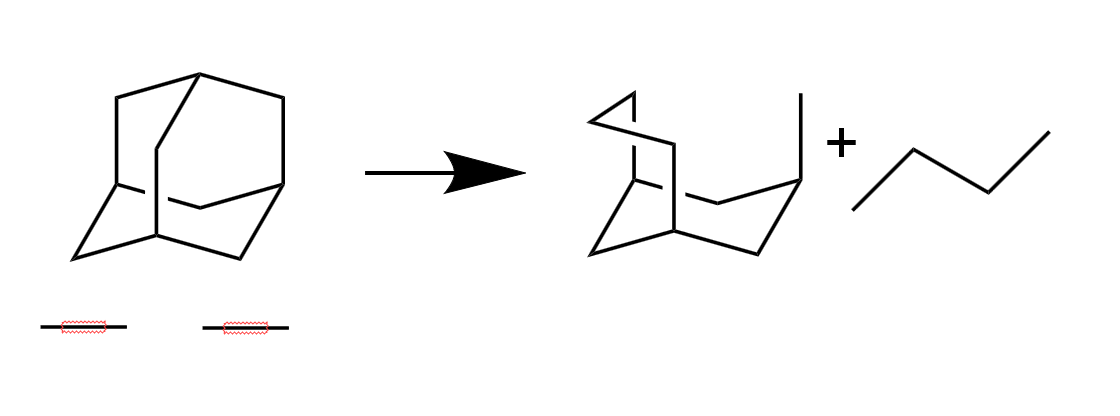
\includegraphics[width=15cm]{reaccion.png} \\
 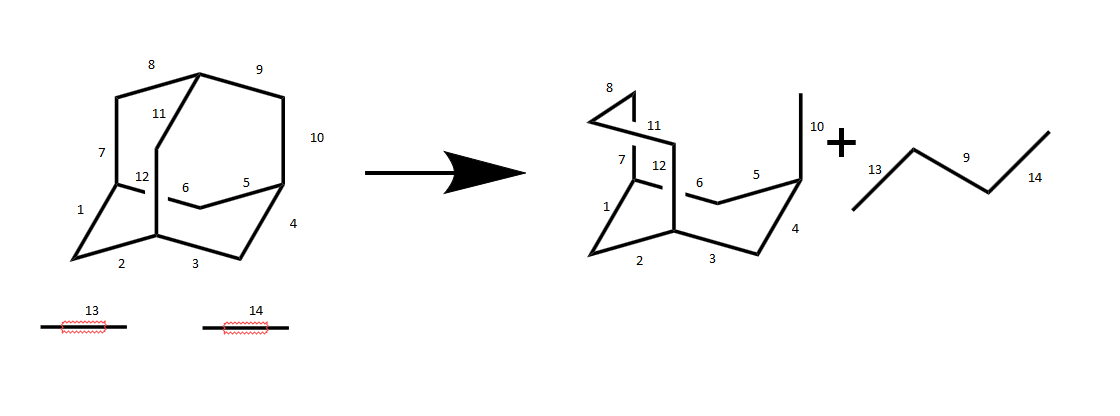
\includegraphics[width=15cm]{reaccion_num_car.png}
\end{figure}

\begin{tabular}{|c|c|}
\hline
{Parte de la ecuación} & {Número de enlaces C-C} \\ \hline
Reactivos & 14 \\ \hline
Productos & 14 \\ \hline

\end{tabular}

\end{document}
